\documentclass{article}
\usepackage[UTF8]{ctex} 
\usepackage{amsmath}
\usepackage{bm}
\usepackage{amssymb}
\usepackage{geometry}
\usepackage{graphicx}
\usepackage{listings}
\usepackage{tikz}
\usetikzlibrary{arrows.meta, positioning, shapes.geometric}
\usetikzlibrary{decorations.pathreplacing, fit}
\geometry{a4paper, margin=1.5cm}

\title{图(1)}
\author{Tan Yiqing}
\date{\today}

\begin{document}
\maketitle
    
    \begin{figure}[h]
        \centering
        \includegraphics[width=0.7\textwidth]{"D:/program/data_construction/firefly/image.png"}
    \end{figure}

\section{定义}
图是由顶点的有穷非空集合和顶点之间边的集合组成,通常表示为:
\begin{equation}
    G = (V, E)
\end{equation}
其中,$V$ 是顶点集合,$E$ 是边集合。\\

其他定义:\\
\begin{enumerate}
    \item 若顶点与顶点之间的边有方向,则称为边为有向边,如果图的任意一条边都有方向,则称为有向图;
否则称为无向边、无向图(任意一条边都无方向)(undirected graph)。
    \item 简单图是指图中不存在重边(同一条边不同时出现)和自环(顶点到自身的边)的图。\\
    \pmb{注意:}有向图方向相反的两条边不视为重边。
    \item 邻接:两个点之间有边相连,则称这两个点是邻接的。\\
    \pmb{有向图}中,若方向是从$v_i$指向$v_j$,则称$v_i$邻接到$v_j$,$v_j$邻接自$v_i$。
    \item 依附:如果一条边连接两个顶点,则称这条边依附于这两个顶点。
    \item 无向完全图:任意两个顶点之间都存在边。
    \item 有向完全图:任意两个顶点之间都存在两条方向相反的边。
    \item 稀疏图和稠密图:如果图中的边数远小于顶点数的平方(边很少),则称为稀疏图,否则称为稠密图。
    \item 顶点的度:无向图中,依附于该顶点的边的数量称为该顶点的度。记为 $TD(v)$ or $deg(v)$。容易证明满足该公式:
    \begin{equation}
        \sum_{i} TD(v) = 2e
    \end{equation}
    \item 出度和入度:有向图中,入度是以该顶点为弧头的弧的数目,记为 $ID(v)$ or $deg^-(v)$;
    出度是以该顶点为弧尾的弧的数目,记为 $OD(v)$ or $deg^+(v)$。其满足该公式:
    \begin{equation}
        \sum_{i} OD(v) = \sum_{i} ID(v) = e
    \end{equation}
    \item 权:对边赋予的有意义的数值量。\\
    \pmb{注意:}哈夫曼树的权重是赋值在叶子节点上的,而不是边上。
    \item 网:边上带权的图。
    \item 路径:无向图中,从顶点$v_i$到顶点$v_j$的一条边的序列,记为:
    \begin{equation}
        P = (v_i, v_{a1}, v_{a2}, ..., v_j)
    \end{equation}
    有向图中,路径也有方向。
    \item 路径长度:非带权图中,路径上边的数目;带权图中,路径上边的权值之和。
    \item 回路(环):起点和终点相同的路径。
    \item 简单路径:路径中没有重复顶点的路径。
    \item 简单回路(简单环):除了起点和终点外,路径中没有重复顶点的回路。
    \item 子图:图$G'=(V', E')$是图$G=(V, E)$的子图,当且仅当$V' \subseteq V$且$E' \subseteq E$。
    \item 连通图(connected graph):无向图中,若两个顶点之间有路径相连,则称这两个点连通;
    若两个顶点之间有路径相连,则称该图为连通图。
    \item 连通分量:无向图中,极大连通子图称为连通分量。可以视作连通图的一个划分。
    \item 强连通图(strongly connected graph):有向图中,若任意两个顶点之间都有路径相连(即$v_i$到$v_j$和$v_j$到$v_i$都有路径),
    则称该图为强连通图。
    \item 强连通分量:非强连通图中,极大强连通子图称为强连通分量。
    \item 生成树:见图(2)
    \item 生成森林:见图(2)
\end{enumerate}

\section{图的遍历}
\indent 图的遍历是指按照某种策略访问图中的每一个顶点和边。常见的图遍历算法有深度优先搜索(DFS)和广度优先搜索(BFS)。
\subsection{DFS}
\indent 基本思想:
\begin{enumerate}
    \item 访问顶点v。
    \item 从v的未被访问的邻接点中选取一个顶点w,递归地对w进行DFS遍历。
    \item 重复步骤2,直到所有顶点都被访问。
\end{enumerate}

\indent 以无向图 $G=(V,E)$ 为例,顶点 $V=\{A,B,C,D,E,F\}$,边
$E=\{(A,B),(A,C),(B,D),(B,E),(C,F)\}$。从 $A$ 出发,按字母序访问未访问邻接点。

\begin{figure}[h]
  \centering
  \begin{tikzpicture}[
    >=Latex, node distance=18mm,
    vertex/.style={circle, draw, thick, minimum size=7mm, align=center},
    el/.style={-Latex, shorten >=2pt, shorten <=2pt, line width=0.6pt}
  ]
    % nodes
    \node[vertex, label=above:{A (1)}] (A) at (0,0) {A};
    \node[vertex, label=left:{B (2)}]  (B) at (-2,-1.8) {B};
    \node[vertex, label=right:{C (5)}] (C) at ( 2,-1.8) {C};
    \node[vertex, label=left:{D (3)}]  (D) at (-3.2,-3.8) {D};
    \node[vertex, label=right:{E (4)}] (E) at (-0.8,-3.8) {E};
    \node[vertex, label=right:{F (6)}] (F) at ( 2.0,-3.8) {F};

    % undirected edges
    \draw (A) -- (B);
    \draw (A) -- (C);
    \draw (B) -- (D);
    \draw (B) -- (E);
    \draw (C) -- (F);

    % start marker
    \node[above=3mm of A] {\small 起点};
  \end{tikzpicture}
  \caption{DFS 示例图与首次访问次序(括号内)}
\end{figure}

访问次序与调用栈(递归)要点(按字母序走未访问邻居):
\begin{enumerate}
  \item 进入 A:栈 [A];首访 A。
  \item A 的首未访邻居 B:入栈 [A,B];首访 B。
  \item B 的首未访邻居 D:入栈 [A,B,D];首访 D;D 无新邻,出栈回到 B:[A,B]。
  \item B 的下一个未访邻居 E:入栈 [A,B,E];首访 E;E 无新邻,出栈回到 B:[A,B];B 完毕,出栈回到 A:[A]。
  \item A 的下一个未访邻居 C:入栈 [A,C];首访 C。
  \item C 的首未访邻居 F:入栈 [A,C,F];首访 F;F 无新邻,出栈回到 C:[A,C];C 完毕出栈回到 A:[A];A 完毕,栈变空 []。
\end{enumerate}


\begin{figure}[h]
\centering
\begin{tikzpicture}[
  >=Latex,
  x=1.6cm, y=6mm, % 统一坐标刻度:横向 1.6cm,纵向 6mm
  stackbox/.style={draw, minimum width=8mm, minimum height=5mm, align=center, font=\scriptsize, inner sep=1pt},
  tlabel/.style={font=\scriptsize, inner sep=1pt}
]
  % 时间刻度标签
  \foreach \i/\x in {0/0,1/1,2/2,3/3,4/4,5/5,6/6,7/7,8/8,9/9,10/10,11/11} {
    \node[tlabel] at (\x,3.4) {$t_{\i}$};
  }

  % 单列栈宏:每步上移 1 个 y 单位(6mm)
    \newcommand{\stackcol}[2]{%
        \begin{scope}[shift={(#1,0)}]
            \draw[gray!50] (-0.7,-0.3) rectangle (0.7,3.2);
            \foreach \yy in {0,...,5} \draw[gray!20] (-0.7,\yy) -- (0.7,\yy);
            \foreach [count=\i] \item in {#2} {%
                \node[stackbox] at (0,{(\i-1)*0.9}) {\item}; % 0.9 可调,增大为 1 或 1.1 拉开距离
            }
        \end{scope}
    }

  % 关键时刻的调用栈(自底向上)
  \stackcol{0}  {A}           % t0
  \stackcol{1}  {A,B}         % t1
  \stackcol{2}  {A,B,D}       % t2
  \stackcol{3}  {A,B}         % t3
  \stackcol{4}  {A,B,E}       % t4
  \stackcol{5}  {A,B}         % t5
  \stackcol{6}  {A}           % t6
  \stackcol{7}  {A,C}         % t7
  \stackcol{8}  {A,C,F}       % t8
  \stackcol{9}  {A,C}         % t9
  \stackcol{10} {A}           % t10
  \stackcol{11} {}            % t11

  \node[tlabel, anchor=west] at (-0.2,-0.7) {注:每列为该时刻递归栈(自底向上)};
\end{tikzpicture}
\caption{DFS 递归调用栈随时间演化(自底向上)}
\end{figure}


\indent 伪代码如下:
\begin{enumerate}
    \item 访问顶点v;visited[v] = 1。
    \item w = 第一个邻接点(v)。
    \item while (w != NULL) 
        \begin{enumerate}
            \item if (visited[w] == 0) 
                \begin{enumerate}
                    \item DFS(w)。
                \end{enumerate}
            \item w = 下一个邻接点(v)。
        \end{enumerate}
\end{enumerate}

\subsection{BFS}
\indent 基本思想:
\begin{enumerate}
    \item 访问顶点v。
    \item 将v的所有未被访问的邻接点加入队列。
    \item 从队列中取出下一个顶点w,递归地对w进行BFS遍历。
    \item 重复步骤2和3,直到队列为空。
\end{enumerate}

\indent 以无向图 $G=(V,E)$ 为例,顶点 $V=\{A,B,C,D,E,F\}$,边
$E=\{(A,B),(A,C),(B,D),(B,E),(C,F)\}$。从 $A$ 出发,按字母序入队未访问邻接点。

\begin{figure}[h]
  \centering
  \begin{tikzpicture}[
    >=Latex, node distance=18mm,
    vertex/.style={circle, draw, thick, minimum size=7mm, align=center},
    el/.style={-Latex, shorten >=2pt, shorten <=2pt, line width=0.6pt}
  ]
    % nodes
    \node[vertex, label=above:{A (1)}] (A) at (0,0) {A};
    \node[vertex, label=left:{B (2)}]  (B) at (-2,-1.8) {B};
    \node[vertex, label=right:{C (3)}] (C) at ( 2,-1.8) {C};
    \node[vertex, label=left:{D (4)}]  (D) at (-3.2,-3.8) {D};
    \node[vertex, label=right:{E (5)}] (E) at (-0.8,-3.8) {E};
    \node[vertex, label=right:{F (6)}] (F) at ( 2.0,-3.8) {F};

    % undirected edges
    \draw (A) -- (B);
    \draw (A) -- (C);
    \draw (B) -- (D);
    \draw (B) -- (E);
    \draw (C) -- (F);

    % start marker
    \node[above=3mm of A] {\small 起点};
  \end{tikzpicture}
  \caption{BFS 示例图与首次访问次序(括号内)}
\end{figure}

访问次序与队列关键状态(按字母序入队未访问邻居):
\begin{enumerate}
  \item $t_0$:队列入队 A,Q=[A]。
  \item $t_1$:出队 A,访问 A;入队 B、C,Q=[B,C]。
  \item $t_2$:出队 B,访问 B;入队 D、E,Q=[C,D,E]。
  \item $t_3$:出队 C,访问 C;入队 F,Q=[D,E,F]。
  \item $t_4$:出队 D,访问 D;Q=[E,F]。
  \item $t_5$:出队 E,访问 E;Q=[F]。
  \item $t_6$:出队 F,访问 F;Q=[],遍历结束。
\end{enumerate}

\begin{figure}[h]
\centering
\begin{tikzpicture}[
  >=Latex,
  x=1cm, y=6mm, % 坐标刻度:列间距用 colw 控制,这里取 1cm/列单位
  queuebox/.style={draw, rounded corners, minimum width=7mm, minimum height=5mm,
                   align=center, font=\scriptsize, inner sep=1pt},
  tlabel/.style={font=\scriptsize, inner sep=1pt}
]
  % 时间刻度标签
  \foreach \i/\x in {0/0,1/1,2/2,3/3,4/4,5/5,6/6} {
    \node[tlabel] at (\x*2.2,2.6) {$t_{\i}$}; % 与列间距一致
  }

    \def\colw{2.2}   % 组与组的列间距
    \def\dx{0.7}     % 同组元素水平间距
    \def\padL{0.5}   % 背景框左侧内边距
    \def\padR{0.5}   % 背景框右侧内边距

    \newcommand{\queuecol}[2]{%
    \begin{scope}[shift={({#1*\colw},0)}]
        % 统计元素个数 n
        \pgfmathtruncatemacro{\n}{0}
        \foreach \_ in {#2} { \pgfmathtruncatemacro{\n}{\n+1} }
        % 计算总宽度与半宽:总宽 = 左内边距 + 右内边距 + (n-1)*dx
        \pgfmathsetmacro{\totalw}{\padL + \padR + max(0, (\n-1)*\dx)}
        \pgfmathsetmacro{\half}{\totalw/2}
        % 背景框
        \draw[gray!50] (-\half,-0.6) rectangle (\half,1.3);
        \node[tlabel, anchor=west] at (-\half+0.05,1.05) {front$\rightarrow$};
        \node[tlabel, anchor=east] at ( \half-0.05,1.05) {$\leftarrow$back};
        % 第一个元素的 x 坐标:左边缘 + 左内边距
        \pgfmathsetmacro{\xfirst}{-\half + \padL}
        % 放置元素:第一个与左边缘对齐(含 padL),其余依次右移 dx
        \foreach \item [count=\j] in {#2} {%
        \pgfmathsetmacro{\xx}{\xfirst + (\j-1)*\dx}
        \node[queuebox] at (\xx,0.2) {\item};
        }
    \end{scope}
    }

  % 各时刻队列内容(队头在左)
  \queuecol{0}  {A}           % t0
  \queuecol{1}  {B,C}         % t1
  \queuecol{2}  {C,D,E}       % t2
  \queuecol{3}  {D,E,F}       % t3
  \queuecol{4}  {E,F}         % t4
  \queuecol{5}  {F}           % t5
  \queuecol{6}  {}            % t6

  \node[tlabel, anchor=west] at (-0.2,-0.9) {注:每列为该时刻队列内容(队头在左)};
\end{tikzpicture}
\caption{BFS 队列随时间演化(队头在左)}
\end{figure}

\indent 伪代码如下:
\begin{enumerate}
    \item 初始化队列Q为空。
    \item 访问顶点v;visited[v] = 1。
    \item 将v入队列Q。
    \item while (Q 不为空) 
        \begin{enumerate}
            \item v = 出队列Q。
            \item u = 第一个邻接点(v)。
            \item while (u != NULL) 
                \begin{enumerate}
                    \item if (visited[u] == 0) 
                        \begin{enumerate}
                            \item 访问顶点u;visited[u] = 1。
                            \item 将u入队列Q。
                        \end{enumerate}
                    \item u = 下一个邻接点(v)。
                \end{enumerate}
        \end{enumerate}
\end{enumerate}

\section{图的存储结构}
\indent 图的存储结构主要有邻接矩阵和邻接表两种方式。
\subsection{邻接矩阵}
\indent 用一个一维数组存储图中顶点的信息。用一个二维数组(邻接矩阵)存储图中各顶点之间的边的信息。\\

\paragraph{示例:无向图的邻接矩阵(vertex 与 arc)}
设顶点集合 $V=\{A,B,C,D\}$,边集合 $E=\{(A,B),(A,C),(B,C),(C,D)\}$。按索引映射
$0\!\to\!A,\ 1\!\to\!B,\ 2\!\to\!C,\ 3\!\to\!D$。

\[
\text{vertex}[0..3] = [A,\ B,\ C,\ D]
\]
\[
\text{arc} =
\begin{bmatrix}
0 & 1 & 1 & 0\\
1 & 0 & 1 & 0\\
1 & 1 & 0 & 1\\
0 & 0 & 1 & 0
\end{bmatrix}
\quad
\begin{array}{l}
\text{arc}[i][j]=1 \iff \text{vertex}[i]\text{ 与 }\text{vertex}[j]\text{有边} \\
\text{无向图矩阵对称;对角线为 }0
\end{array}
\]

\begin{figure}[h]
\centering
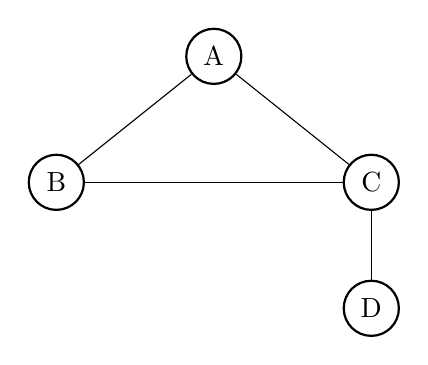
\begin{tikzpicture}[
  >=Latex, node distance=16mm,
  vertex/.style={circle, draw, thick, minimum size=7mm, align=center}
]
  \node[vertex] (A) at (0,0) {A};
  \node[vertex] (B) at (-2,-1.6) {B};
  \node[vertex] (C) at ( 2,-1.6) {C};
  \node[vertex] (D) at ( 2,-3.2) {D};

  \draw (A)--(B);
  \draw (A)--(C);
  \draw (B)--(C);
  \draw (C)--(D);
\end{tikzpicture}
\caption{对应的无向图示意(A-B, A-C, B-C, C-D)}
\end{figure}

\noindent 矩阵读法示例:$\text{arc}[0][1]=1$ 表示 $A$ 与 $B$ 相邻;$\text{arc}[3][0]=0$ 表示 $D$ 与 $A$ 不相邻。


\indent 邻接矩阵的数学性质:
\begin{enumerate}
    \item 对角线全为0。
    \item 第i行非零元素个数等于顶点$i$的度。
    \item 无向图的邻接矩阵是对称矩阵,有向图则矩阵一般不对称(除了完全图)。
    \item arc[i][j] == 1代表顶点i和顶点j之间有边相连,否则没有边相连。
    \item 扫描第i行可以找出与顶点i邻接的所有顶点。
    (有向图出度为第i行元素之和,入度为第i列元素之和)
\end{enumerate}

\indent 网图的邻接矩阵:
\[
    \text{arc} = 
    \begin{cases}
        w_{ij}, & \text{if } (i,j) \in E \\
        0, & \text{if } i = j \\
        \infty, & \text{otherwise}
    \end{cases}
\]

\subsection{邻接表}
\indent 见图(2)

\end{document}